\documentclass[master=cws,masteroption=se]{kulemt}
\setup{title={DevOps: Operational data for developers},
  author={Stef Van Gils},
  promotor={Prof.\ W. Joosen},
  assessor={Dimitri Van Landuyt},
  assistant={Dimitri Van Landuyt}}
% De volgende \setup mag verwijderd worden als geen fiche gewenst is.
\setup{filingcard,
  translatedtitle={DevOps: Operational data for developers},
  udc=621.3,
  shortabstract={}}
% Verwijder de "%" op de volgende lijn als je de kaft wil afdrukken
%\setup{coverpageonly}
% Verwijder de "%" op de volgende lijn als je enkel de eerste pagina's wil
% afdrukken en de rest bv. via Word aanmaken.
%\setup{frontpagesonly}

% Kies de fonts voor de gewone tekst, bv. Latin Modern
\setup{font=lm}

% Hier kun je dan nog andere pakketten laden of eigen definities voorzien

% Tenslotte wordt hyperref gebruikt voor pdf bestanden.
% Dit mag verwijderd worden voor de af te drukken versie.
\usepackage[pdfusetitle,colorlinks,plainpages=false]{hyperref}

%%%%%%%
% Om wat tekst te genereren wordt hier het lipsum pakket gebruikt.
% Bij een echte masterproef heb je dit natuurlijk nooit nodig!
\IfFileExists{lipsum.sty}%
 {\usepackage{lipsum}\setlipsumdefault{11-13}}%
 {\newcommand{\lipsum}[1][11-13]{\par Hier komt wat tekst: lipsum ##1.\par}}
%%%%%%%

%%%%%%%
% Gebruikt om \texttt{} line breaks uit te voeren indien nodig
\newcommand*\justify{%
  \fontdimen2\font=0.4em% interword space
  \fontdimen3\font=0.2em% interword stretch
  \fontdimen4\font=0.1em% interword shrink
  \fontdimen7\font=0.1em% extra space
  \hyphenchar\font=`\-% allowing hyphenation
}
%%%%%%%

%\includeonly{hfdst-n}
\begin{document}

\begin{preface}
  Dit is mijn dankwoord om iedereen te danken die mij bezig gehouden heeft.
  Hierbij dank ik mijn promotor, mijn begeleider en de voltallige jury.
  Ook mijn familie heeft mij erg gesteund natuurlijk.
\end{preface}

\tableofcontents*

\begin{abstract}
  In dit \texttt{abstract} environment wordt een al dan niet uitgebreide
  samenvatting van het werk gegeven. De bedoeling is wel dat dit tot
  1~bladzijde beperkt blijft.

  \lipsum[1]
\end{abstract}

% Een lijst van figuren en tabellen is optioneel
%\listoffigures
%\listoftables
% Bij een beperkt aantal figuren en tabellen gebruik je liever het volgende:
\listoffiguresandtables
% De lijst van symbolen is eveneens optioneel.
% Deze lijst moet wel manueel aangemaakt worden, bv. als volgt:

% Nu begint de eigenlijke tekst
\mainmatter

%\chapter{Inleiding}
\label{inleiding}
In dit hoofdstuk wordt het werk ingeleid. Het doel wordt gedefinieerd en er
wordt uitgelegd wat de te volgen weg is (beter bekend als de rode draad).

Als je niet goed weet wat een masterproef is, kan je altijd
Wikipedia\cite{wiki} eens nakijken.

\section{Lorem ipsum 4--5}
\lipsum[4-5]

\section{Lorem ipsum 6--7}
\lipsum[6-7]

%%% Local Variables: 
%%% mode: latex
%%% TeX-master: "masterproef"
%%% End: 

%\include{hfdst-1}
\include{architectuur}
\include{implementatie}
% ... en zo verder tot
%\chapter{Het laatste hoofdstuk}
\label{hoofdstuk:n}
Een hoofdstuk behandelt een samenhangend geheel dat min of meer op zichzelf
staat. Het is dan ook logisch dat het begint met een inleiding, namelijk
het gedeelte van de tekst dat je nu aan het lezen bent.

\section{Eerste onderwerp in dit hoofdstuk}
De inleidende informatie van dit onderwerp.

\subsection{Een item}
De bijbehorende tekst. Denk eraan om de paragrafen lang genoeg te maken en
de zinnen niet te lang.

Een paragraaf omvat een gedachtengang en bevat dus steeds een paar zinnen.
Een paragraaf die maar \'e\'en lijn lang is, is dus uit den boze.

\section{Tweede onderwerp in dit hoofdstuk}
Er zijn in een hoofdstuk verschillende onderwerpen. We zullen nu
veronderstellen dat dit het laatste onderwerp is.

\section{Besluit van dit hoofdstuk}
Als je in dit hoofdstuk tot belangrijke resultaten of besluiten gekomen
bent, dan is het ook logisch om het hoofdstuk af te ronden met een
overzicht ervan. Voor hoofdstukken zoals de inleiding en het
literatuuroverzicht is dit niet strikt nodig.

%%% Local Variables: 
%%% mode: latex
%%% TeX-master: "masterproef"
%%% End: 

%\chapter{Besluit}
\label{besluit}


In deze thesis is er op zoek gegaan naar een oplossing om het ontwikkelen van mobiele applicaties en de concepten van DevOps te combineren. Er is gekozen om te kijken naar het monitoring aspect van DevOps. Er zijn enkele oplossingen voorgesteld om mobiele applicaties te monitoren, namelijk: built-in OS support, een dedicated test environment en een monitoring library. Uit deze voorstellen is \'e\'en voorstel gekozen, namelijk een library om in een mobiele applicatie in te bouwen die de applicatie monitort. In het doelstellingen hoofdstuk is beschreven welke specificaties de library minimaal moet hebben om een succesvolle library te kunnen zijn. De vormgeving en architectuur van de monitoring library wordt voorgesteld in het architectuur hoofdstuk samen met enkele uitbreidingen op de library. Deze architectuur is ge\"implementeerd in een library die ontwikkeld is voor iOS, het besturingssysteem voor mobiele toestellen van Apple. Deze implementatie is ten slotte ge\"evalueerd om te kijken of deze implementatie kan werken in de realiteit. \\


In het hoofdstuk doelstellingen \ref{doelstelling} zijn een aantal doelstellingen opgesomd voor de ontwikkelde library. Deze werden opgedeeld in volgende categorie\"en: 
\begin{itemize}
\item performance impact
\item schaalbaarheid
\item bruikbaarheid
\item beschikbaarheid
\end{itemize}

\paragraph{De performance impact} werd gezien als het belangrijkste aspect in het ontwikkelen van een monitoring library. Deze impact is onderzocht en getest in het evaluatie hoofstuk \ref{evaluatie}. Uit deze evaluatie kan afgeleid worden dat de impact van de library op een mobiele applicatie klein genoeg is om de applicatie niet significant te vertragen. \\


\paragraph{De schaalbaarheid} van de Tracklytics library is besproken in het evaluatie hoofdstuk \ref{evaluatie}. De back end is het deel van de library dat schaalbaar moet zijn om de requests die van de mobiele library komen te verwerken. De bottleneck in de back end is de relationele database. Deze moet zo goed mogelijk uitgeschaald worden om aan de requests te kunnen voldoen. Een alternatief is om de relationele database te veranderen naar een NoSQL of andere schaalbare database. Het is ook mogelijk voor de developer om de back end op de eigen servers te draaien om zo alle data in eigen bezit te hebben en niet afhankelijk te zijn van de Tracklytics infrastructuur.\\


\paragraph{De bruikbaarheid} van de library wordt gedefini\"eerd als hoeveel moeite een developer nodig heeft om de library in te bouwen in de mobiele applicatie. In het evaluatie hoofdstuk \ref{evaluatie} is nagegaan hoeveel moeite een developer nodig heeft om de library in de applicatie in te bouwen. In deze evaluatie zijn de volgende zaken opgenomen: de totale tijd om de library in te bouwen, het aantal lijnen code en wat er gemonitord wordt door de library. Uit de gegevens die hieruit zijn gekomen kan geconcludeerd worden dat de developer effort minimaal is.

\paragraph{Om de beschikbaarheid} van de data maximaal te houden moet elke meting naar de back end verstuurd worden. De Tracklytics library laat de keuze of de data tijdelijk op de harde schijf van het toestel opgeslagen moet worden over aan de developer zelf. De developer moet deze keuze aangeven in het dashboard. \\

De voorgaande paragrafen tonen aan dat de doelstellingen vooropgesteld in deze thesis voldaan zijn in de implementatie van de library. Naast deze doelstellingen werd in het hoofdstuk over architectuur \ref{architectuur} nog enkele vereisten gegeven waaraan de library moet voldoen om de developer te helpen bij het ontwikkelen van een mobiele applicatie, namelijk: 
\begin{itemize}
\item Op welke buttons/switches/entry in een tabel gebruikers drukken
\item Welke schermen de gebruikers bezoeken
\item Het gemiddeld aantal zoekresultaten per zoekopdracht
\item Het gemiddelde of de verdeling van het getal dat een gebruiker in een bepaald veld invoert
\item Hoe lang de applicatie gemiddeld gebruikt wordt
\item Hoe lang een stuk code over het uitvoeren ervan doet om na te gaan of deze code niet te traag is.
\item De tijd die een request over het internet nodig heeft om te voltooien om te kijken of er hier een vertraging opgelopen wordt.
\item Het gemiddeld aantal entries in een array of een NSDictionary (een Map in Java). Indien er ge\"itereerd wordt over deze datastructuren kan een groot aantal entries ervoor zorgen dat dat stuk code de applicatie vertraagt.
\item Het gemiddeld aantal keer dat een bepaalde methode uitgevoerd wordt om te kijken
\end{itemize}

Met behulp van de Tracklytics library kan aan deze vereisten voldaan worden. De eerste twee vereisten kunnen ingelost worden door counters in te bouwen in de applicatie. De tweede, derde, voorlaatste en laatste vereiste kunnen opgelost worden door ofwel een gauge te gebruiken ofwel een histogram te gebruiken. Aan de vierde, de vijfde en de zesde vereiste kan voldaan worden door een timer in te bouwen in de applicatie.\\

Tijdens het oplossen van deze doelstellingen en het ontwikkelen van de Tracklytics library zijn er enkele problemen opgetreden. Allereerst was het moeilijk om uit te denken wat er gemonitord zou moeten worden en welke types van meetobjecten er in de library ge\"implementeerd moesten worden. Het was daarnaast moeilijk om deze types meetobjecten om te zetten in een performante mobiele library die bruikbaar kon zijn in de realiteit. Het opstellen van nuttige testopstellingen was een moeilijkheid, omdat we de impact van de library zo goed mogelijk wouden testen.\\

Naast het ontwikkelen van de mobiele applicatie was het ontwikkelen van het dashboard de grote moeilijkheid. Allereerst is er uitgezocht hoe we de verschillende meetobjecten het beste kunnen weergeven. Deze weergave is getweakt tot we dachten dat het de beste weergave was die we de developers konden geven. Daarnaast heeft het ontwikkelen van dit dashboard veel tijd gekost. Enerzijds omdat web development relatief nieuw voor mij was en anderzijds omdat er complexe geneste lussen zitten in het ophalen van de data bij de detail pagina's. \\

Een monitoring library heeft zijn voor- en nadelen. De gebruikers kunnen de applicatie anders gebruiken dan dat deze getest is in een test opstelling. Een monitoring library kan deze informatie ophalen, omdat deze in de applicatie, die in productie is, ingebouwd is. Het nadeel aan een monitoring library is dat deze een extra performance impact heeft op de applicatie, maar zoals eerder besproken is deze impact klein genoeg. Het dashboard zou nog wat meer functionaliteit kunnen hebben door nog gedetailleerdere overzichten te geven of extra mogelijkheden te geven tot het verkleinen van de dataset. \\

Indien ik meer tijd zou hebben gehad in het ontwikkelen van deze thesis zou ik graag nog wat uitbreidingen toegevoegd hebben aan de monitoring library. Als eerste zou ik graag het tracken van features hebben toegevoegd aan de applicatie. Features zijn een samenhang van componenten die een functie uitvoeren. Naar dit soort tracking van applicaties is momenteel veel onderzoek naar en ik zou dit onderzoek willen combineren met mobiele applicaties. \\
Daarnaast zou ik graag AB testing in de applicatie inbouwen. AB testing is het concept dat een selecte groep van de gebruikers een nieuwere versie te zien krijgen dan een andere groep. Zo kan de uitrol van een nieuwe versie geleidelijk aan gebeuren en indien er een bug zit in de software is deze enkel zichtbaar voor een klein deel van de gebruikers. In mobiele applicaties is dit een uitdaging, omdat dynamisch code laden niet mogelijk is. Ik zou willen onderzoeken wat de mogelijkheden hierin zijn en welke alternatieven er zijn om toch aan AB testing te kunnen doen en deze dan combineren met de monitoring library.\\
Ten slotte zou ik willen onderzoeken of het mogelijk is om een plugin te bouwen voor Xcode, de ontwikkelingsomgeving voor het iOS besturingssysteem. Deze plugin zou de developer kunnen helpen met het ontwikkelen van de library door bijvoorbeeld automatisch aan te geven welke stukken code het traagste zijn en hoe traag op basis van de metingen door de Tracklytics library. \\
 
%%% Local Variables: 
%%% mode: latex
%%% TeX-master: "masterproef"
%%% End: 


% Indien er bijlagen zijn:
%\appendixpage*          % indien gewenst
%\appendix
%\chapter{IEEE Artikel}
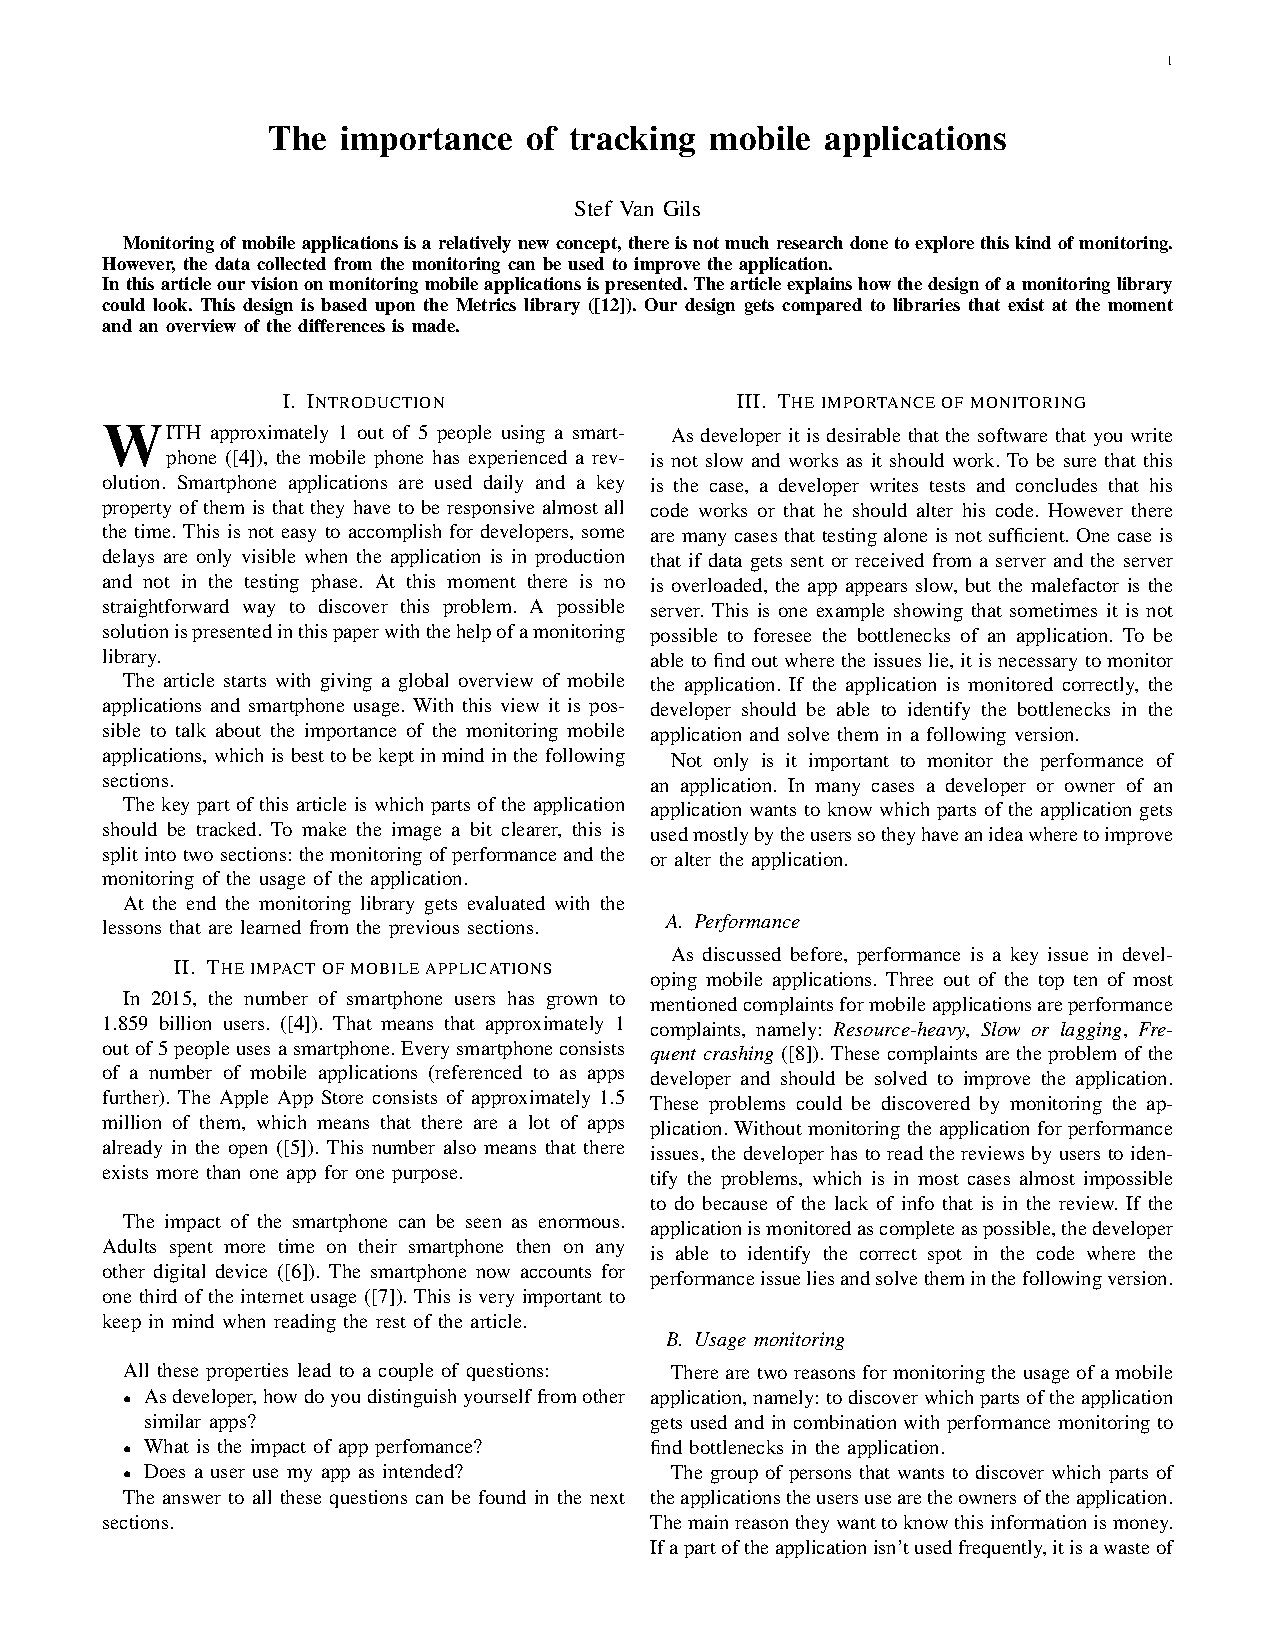
\includepdf[pages={1-5}]{article_thesis}
% ... en zo verder tot
%\chapter{De laatste bijlage}
\label{app:n}
In de bijlagen vindt men de data terug die nuttig kunnen zijn voor de
lezer, maar die niet essentieel zijn om het betoog in de normale tekst te
kunnen volgen. Voorbeelden hiervan zijn bronbestanden,
configuratie-informatie, langdradige wiskundige afleidingen, enz.

\section{Lorem 20-24}
\lipsum[20-24]

\section{Lorem 25-27}
\lipsum[25-27]

%%% Local Variables: 
%%% mode: latex
%%% TeX-master: "masterproef"
%%% End: 


\backmatter
% Na de bijlagen plaatst men nog de bibliografie.
% Je kan de  standaard "abbrv" bibliografiestijl vervangen door een andere.
\bibliographystyle{abbrv}
\bibliography{referenties}



\end{document}

%%% Local Variables: 
%%% mode: latex
%%% TeX-master: t
%%% End: 
